\chapter{Performance Analysis}

In this section, we present the results of our proposed acceleration techniques and describe the fitness function used across all experiments. The goal of our fitness function is to balance predictive performance with hardware efficiency, ensuring that the selected models are not only accurate but also suitable for deployment on resource-constrained devices.

The fitness function is defined as:

\begin{equation}
\text{Fitness} =
\begin{cases}
\begin{aligned}
0.7 \cdot \text{Accuracy}_{\text{TFLite}} 
+ 0.2 \cdot \left(1 - \dfrac{\text{RAM}}{\text{MaxRAM}}\right) \\
+ 0.1 \cdot \left(1 - \dfrac{\text{Flash}}{\text{MaxFlash}}\right),
\end{aligned}
& \text{if } \text{RAM} \leq \text{MaxRAM} \land \text{Flash} \leq \text{MaxFlash} \\
-1000, & \text{otherwise}
\end{cases}
\label{eq:fitness_function}
\end{equation}



This formulation was chosen to explicitly incorporate hardware constraints into the optimization objective. Including this fitness function, we effectively guide the Genetic Algorithm (GA) to prioritize models that are not only accurate but also memory-efficient.

Notably, although the highest accuracy achieved during training (at 70 epochs) was approximately 60\%, the fitness function allows models with lower accuracy (e.g., around 40\%) to outperform others if they demonstrate significantly lower memory usage. However, by assigning a higher weight (0.7) to the accuracy term in the fitness function, we ensure that performance remains the primary objective. This is especially important considering that accuracy typically ranges from 0.3 to 0.65, while the normalized RAM and Flash components can span from 0 to 0.85. Without the weighted terms, the smallest models would consistently dominate the selection process—regardless of their predictive performance. The chosen weighting strategy ensures that the evolutionary search favors architectures that are not only compact and efficient but also sufficiently accurate for deployment.

It's important to note that microcontrollers are typically designed for specific tasks within embedded systems, combining processing, memory, and input/output peripherals on a single chip. This design makes them cost-effective and power-efficient for dedicated applications . In such scenarios, as long as the model fits within the available memory constraints of the microcontroller, such as the 256KB SRAM of the Arduino Nano 33 BLE Sense , the exact memory consumption becomes less critical. Therefore, the fitness function's weighting ensures a balance between model accuracy and resource efficiency, aligning with the practical considerations of deploying models on resource-constrained devices \cite{arduino_nano33ble}.



\section{Memory Estimation Experiment}
\label{sec:memory_estimation_experiment}
To assess the effectiveness of the proposed memory-aware optimization, a dedicated experiment was conducted in which the memory filtering mechanism was deliberately disabled. In this configuration, models exceeding the allowable RAM or flash memory constraints were not filtered out prior to training. Instead, any model violating the hardware limits was penalized post-training by assigning it a fixed fitness value of –1000. The purpose of this experiment was to investigate whether the genetic algorithm (GA) could inherently learn to avoid infeasible models, despite the lack of preemptive filtering.

Following a 4-hour NAS run, it became evident that only a limited number of models were successfully trained. This was primarily due to the fact that models with larger RAM and flash memory requirements consumed significantly more computational time—even for short training durations. In some cases, a single large model required up to four times the training time of a smaller, resource-efficient one (see Table~\ref{tab:taku_models}). This disparity in training time illustrates the inefficiency introduced by allowing oversized models to enter the search process.

Moreover, after evaluating all trained models, only a small fraction were found to be deployable on the Arduino Nano. While the RankNet-based predictor demonstrated some ability to identify promising architectures before training, its utility was limited in scenarios where the vast majority of candidates were infeasible. Specifically, when many models received the same penalty score (e.g., –1000), the RankNet network struggled to make meaningful comparisons during pairwise ranking. This led to stagnation in the learning process, as the predictor could not effectively differentiate between models based solely on invalid fitness values.

As illustrated in Figure~\ref{fig:memoryEstimationTest}, approximately \textbf{75\%} of the trained models were ultimately undeployable due to violating memory constraints. This result highlights the substantial inefficiencies introduced when memory-aware filtering is not applied. Beyond wasting training time on models that will later be discarded, the overall search process is slowed due to longer training cycles and increased difficulty in selecting promising candidates. Incorporating early memory estimation not only improves the efficiency of NAS by avoiding wasted computation, but also ensures that the evolutionary search is guided more effectively toward viable, deployable solutions.

\clearpage

\begin{table}[ht]
\noindent % removes indentation
\hspace*{-\oddsidemargin} % shift left based on page margin
\makebox[\linewidth][l]{%
\resizebox{1.20\textwidth}{!}{%
\begin{tabular}{|l|c|c|c|c|c|c|c|c|c|c|c|c|c|c|c|}
\hline
\textbf{Model} & \textbf{Train Acc} & \textbf{Test Acc} & \textbf{SWA Acc} & \textbf{TFLite Acc} & \textbf{Opt.} & \textbf{Precision} & \textbf{Recall} & \textbf{F1} & \textbf{RAM (KB)} & \textbf{Flash (KB)} & \textbf{TFLite (KB)} & \textbf{FLOPs} & \textbf{Fitness} & \textbf{Time (min)} & \textbf{Epochs} \\
\hline
TakuNet\_Init\_0 & 0.8922 & 0.5717 & 0.5717 & 0.5730 & adamw & 0.5712 & 0.5717 & 0.5690 & 546.91 & 15020.00 & 13731.02 & 31824133 & -1000.00 & 14.48 & 10 \\
TakuNet\_Mutant\_13 & 0.4719 & 0.4396 & 0.4396 & 0.4367 & adamw & 0.4342 & 0.4396 & 0.4304 & 52.18 & 316.71 & 321.56 & 750018 & 0.5130 & 4.92 & 10 \\
\hline
\end{tabular}
}}
\caption{Summary of two TakuNet models.}
\label{tab:taku_models}
\end{table}

\bigskip

\begin{figure}[ht]
    \centering
    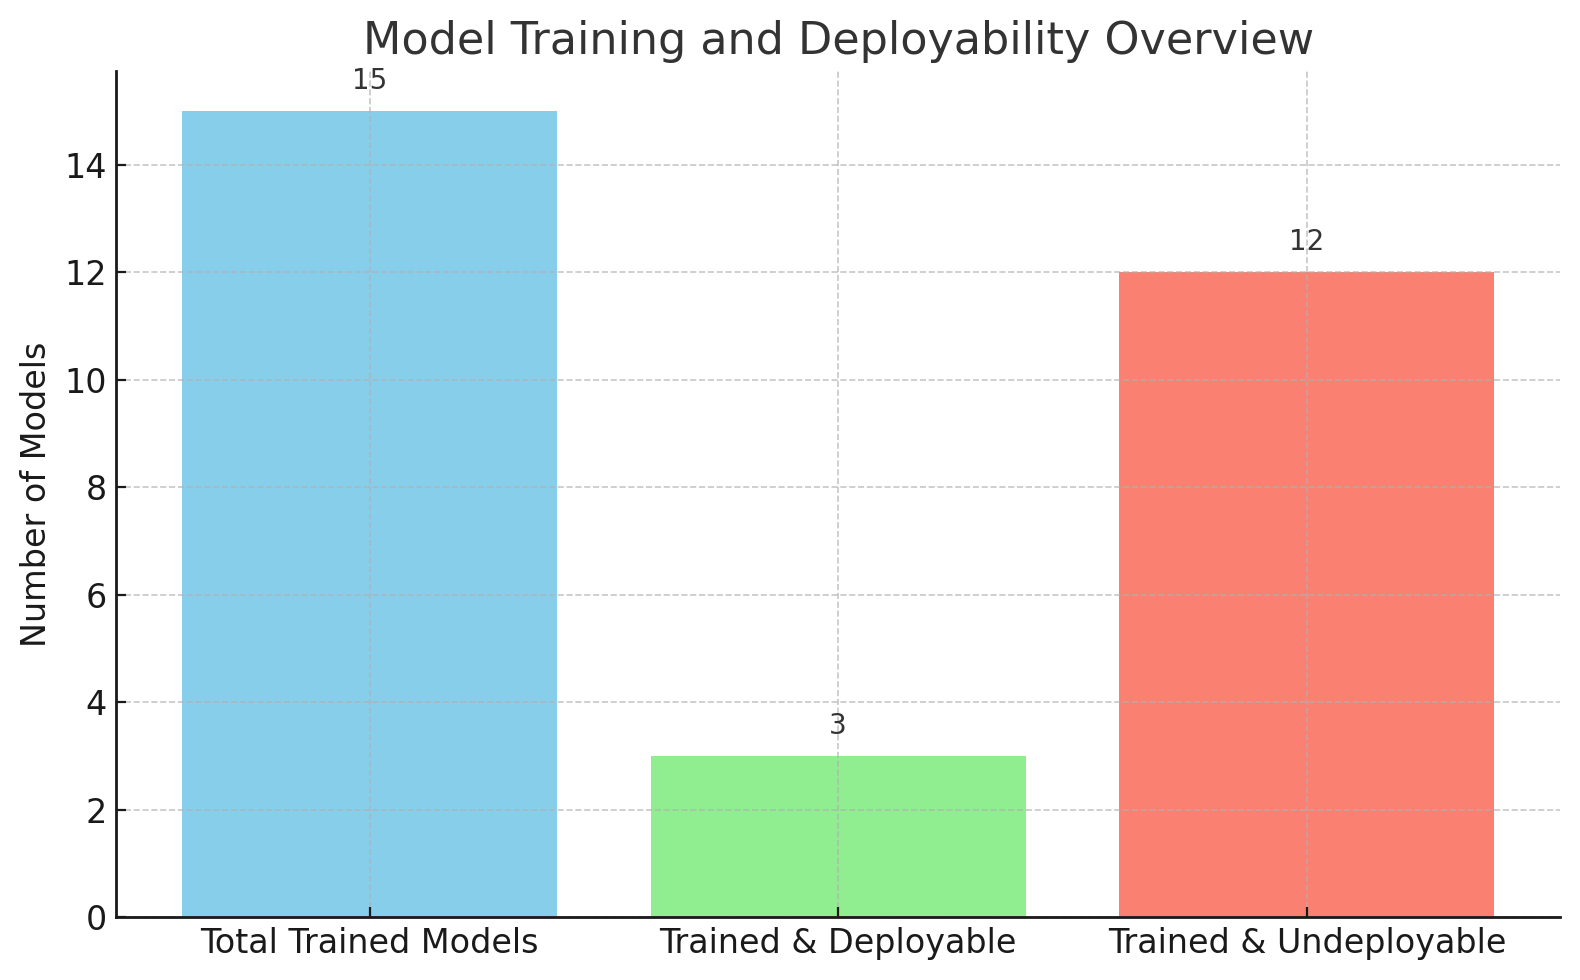
\includegraphics[width=0.85\linewidth]{Pictures/MemoryEstimationTest.png}
    \caption{MemoryEstimationTest}
    \label{fig:memoryEstimationTest}
\end{figure}





\section{RankNet Experiment}
\label{sec:ranknet_experiment}
In this experiment, we analyzed the outcomes of a large-scale NAS run that lasted approximately 9 hours. Given that our selection process is based on tournament comparisons, it is nearly impossible to recreate the exact pairwise matchups observed during the original run. To ensure transparency and reproducibility, we retained both the fitness scores and the parameter configurations of every model evaluated.

To assess the predictive power of the RankNet model, we performed \textbf{10,000 random pairwise comparisons} between different architectures. The task was to determine which of the two models in each pair would perform better. Despite the inherent randomness of such comparisons (where random guessing would yield 50\% accuracy), RankNet correctly predicted the better-performing model \textbf{65\% of the time}.

Although this result may seem modest, a 15-percentage-point improvement over chance is significant in such settings. Even small gains above random chance can yield substantial advantages in optimization tasks \cite{freund1999large}.

It is worth noting that RankNet was trained on only a limited number of samples, making its performance particularly impressive and suggesting that further training could lead to even greater predictive accuracy.

Moreover, in our NAS algorithm, RankNet's potential misjudgments are inherently mitigated. Specifically, we rely on RankNet's predictions only when neither of the competing models has been trained yet. This strategic usage ensures that the actual impact of any prediction error is reduced, and the overall effectiveness of the NAS procedure remains robust—even more so than what is reflected in this isolated evaluation.

While it is difficult to precisely quantify the overall speedup gained by integrating RankNet into the NAS process, the fact that it performs better than random guessing is already valuable. By more accurately identifying promising architectures early on, RankNet helps to avoid the training of clearly suboptimal models. This selective approach evidently contributes to reducing the total time and computational cost required by the NAS algorithm.


\section{Early Stoppage Experiment}
In this experiment, building upon previous observations, we aimed to stop the training of specific models early in order to reduce computational cost when it was likely that their final performance would be suboptimal. As previously discussed, the first few epochs of training tend to be the most informative. If a model fails to reach a predefined validation accuracy threshold by a given cutoff epoch, it is unlikely to outperform others later on. To exploit this, we designed a threshold-based early stopping strategy: during training, if the validation accuracy at a predefined cutoff epoch does not surpass a certain threshold, the training is terminated early. This approach simulates an informed pruning of underperforming models.

To evaluate the effectiveness of this method, we performed a grid search over various cutoff epochs and validation accuracy thresholds. For each configuration, we computed the estimated fitness using a normalized function that incorporates accuracy, RAM usage, and flash memory requirements (see Equation~\ref{eq:fitness_function}). We then used a tournament-style comparison to evaluate how closely these early estimates matched the final results of fully trained models. The configurations were assessed based on their prediction error rate and the total training time saved.

As shown in Table~\ref{tab:early_stopping_results}, the best configuration with an error rate below 25\% achieved a training time reduction of up to 91.4\%. This demonstrates that a well-calibrated threshold-based early stopping strategy can substantially reduce training costs with minimal impact on model selection accuracy.


\begin{table}[H]
\centering
\caption{Top 10 early stopping configurations ranked by time saved.}
\label{tab:early_stopping_results}
\begin{tabular}{cccccc}
\toprule
Cutoff Epoch & Threshold & Error Rate (\%) & Time Saved (min) & Time Saved (\%) \\
\midrule
5 & 0.39 & 26.48 & 508.43 & 91.43 \\
5 & 0.37 & 40.69 & 413.28 & 74.32 \\
\vdots & \vdots & \vdots & \vdots & \vdots \\
\bottomrule
\end{tabular}
\end{table}



\section{Performance Stop Experiment}
In this experiment, we conducted a full 10-hour training run \textbf{without} applying the performance stop optimization described in Section~\ref{sec:performance_stop}.

Figure~\ref{fig:performanceStop} illustrates the proportion of models that could have been early-stopped, along with their corresponding projected loss in validation accuracy. This loss is calculated relative to the highest validation accuracy achieved by any model across all training experiments, thus providing a consistent global benchmark.

As depicted in the figure, approximately 10\% of the models incurred less than a 5\% loss in validation accuracy compared to the best-performing model. Moreover, 30\% and 55\% of the models stayed within 10\% and 20\% of the best, respectively. Remarkably, 90\% of the models remained within a 30\% margin, demonstrating that the majority of early-stopped models still maintained competitive performance.

To evaluate the efficiency gains of this approach, we estimated the training time that could have been saved by applying performance-based early stopping. Assuming a uniform epoch duration per model, a total of \textbf{604 epochs} could have been avoided, translating to approximately \textbf{244.2 minutes} of compute time. This corresponds to nearly \textbf{4 hours} saved out of the total \textbf{556.10 minutes} training time an impressive \textbf{56\%} reduction in computational cost.

To assess the trade-off in decision quality, we conducted a series of random pairwise comparisons between models using both their original and stopped validation accuracy in the fitness evaluation. Across \textbf{10,000 comparisons}, we observed that approximately \textbf{2,100} resulted in incorrect decisions when relying on the stopped accuracy. This yields a decision error rate of \textbf{27\%}, which we consider an acceptable compromise given the substantial gain in the speedup.

These findings support the effectiveness of performance-based early stopping in significantly reducing computational time while preserving acceptable accuracy. In practice, tolerating small projected performance losses can greatly enhance scalability and responsiveness in large-scale evolutionary or model selection tasks.


\begin{figure}[H]
    \centering
    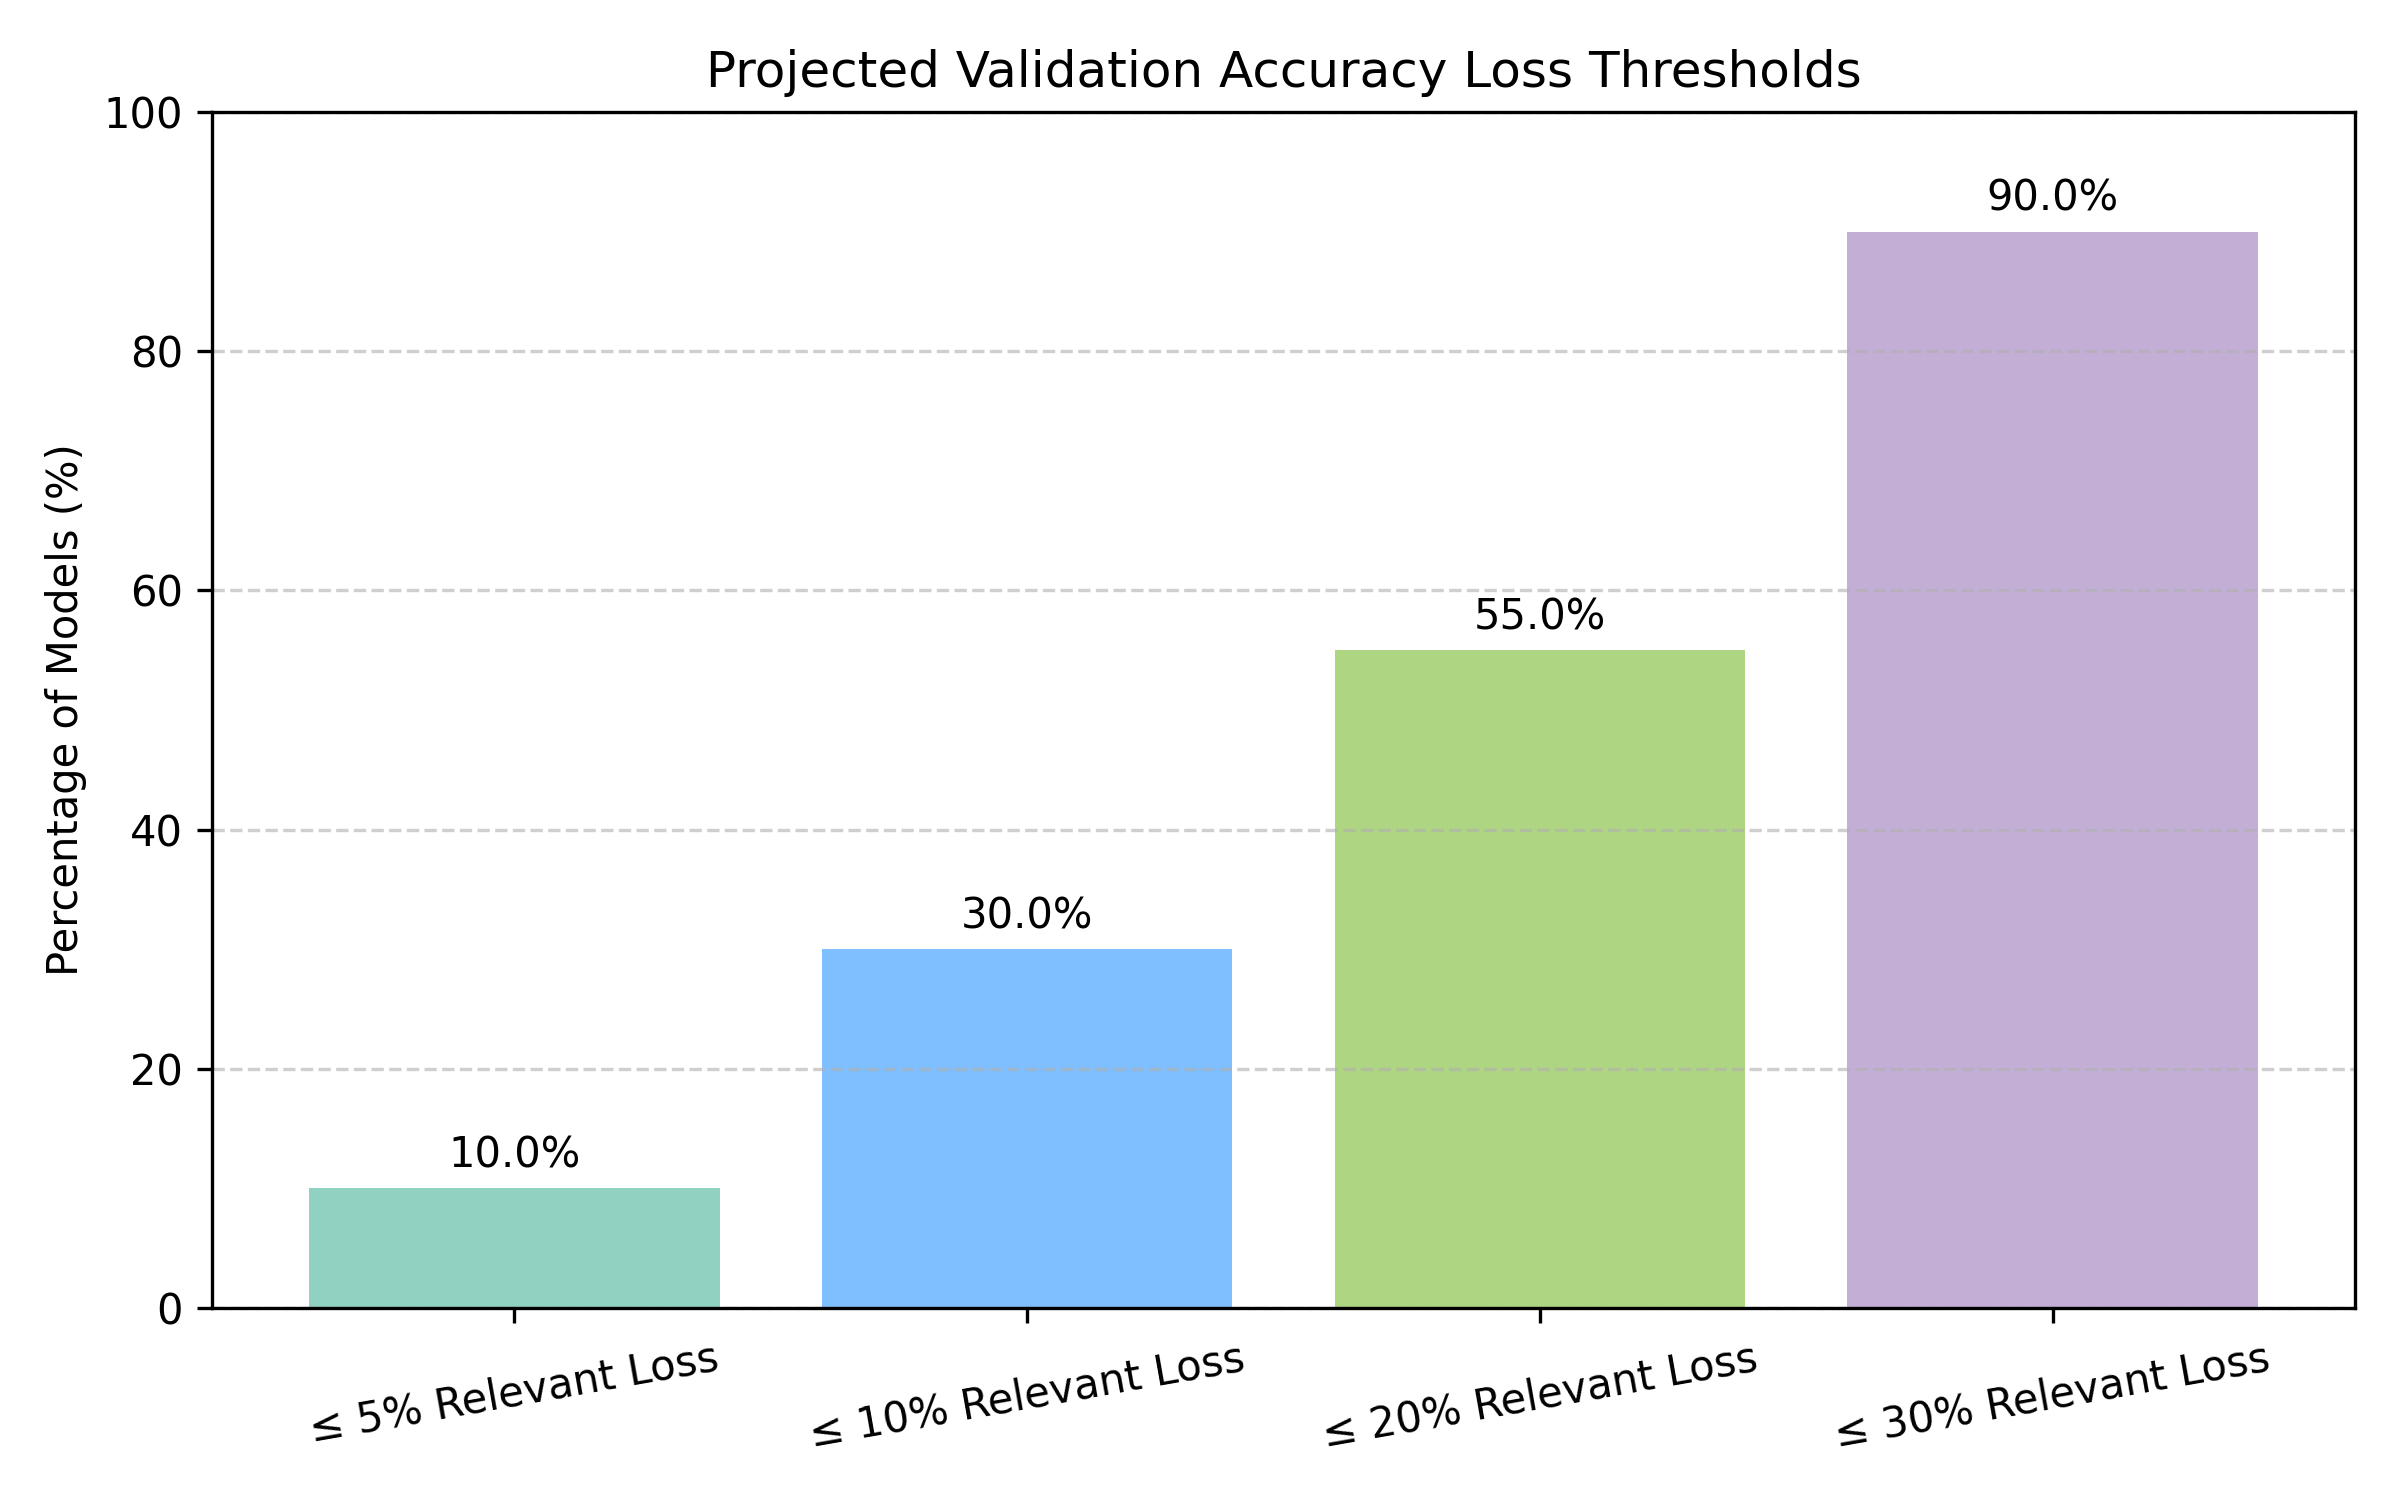
\includegraphics[width=0.85\linewidth]{Pictures/val_accuracy_loss_percentages.png}
    \caption{Percentage of models falling under various thresholds of projected validation accuracy loss relative to the best observed model.}
    \label{fig:performanceStop}
\end{figure}



\section{Learning Rate Experiment}

As previously discussed, cosine learning rate decay is theoretically expected to converge faster than traditional schedules such as \textbf{Step Decay}, \textbf{Constant Learning Rate}, or \textbf{Linear Decay} \cite{li2019exponential}  \cite{kim2021automated}. The motivation behind this experiment is to investigate whether we can achieve reliable performance predictions with fewer than the 70 training epochs we currently use as a baseline.

To test this hypothesis, we selected a set of models that were originally trained for 70 epochs. These models were then \textit{re-trained from scratch} using the cosine decay schedule but with \textbf{reduced epoch budgets}: specifically 10, 20, 30, and 50 epochs. For each of these training durations, we performed \textbf{10,000 random pairwise comparisons} to assess whether early-stopped models could still accurately reflect performance rankings.


\begin{table}[h]
\centering
\begin{tabular}{|c|c|c|p{6cm}|}
\hline
\textbf{Epochs} & \textbf{Prediction Mistake} & \textbf{Avg. Time Reduction} & \textbf{Notes} \\
\hline
10 & $\sim$30\% & $\sim$85.24\% & Fastest training, but leads to high prediction errors and noisy rankings due to underfitting. \\
20 & $\sim$21\% & $\sim$62.12\% & Noticeable improvement in prediction stability; still some inconsistency, but a clear step up from 10 epochs. \\
30 & $\sim$16\% & $\sim$55\% & Achieves competitive accuracy, close to longer trainings; a strong compromise between performance and efficiency. \\
50 & $\sim$15\% & $\sim$32.69\% & Very stable predictions with minimal mistakes; however, the time savings are significantly reduced. \\
\hline
\end{tabular}
\caption{Comparison of RankNet pairwise accuracy using different training durations with cosine decay}
\label{tab:cosine_decay_results}
\end{table}

\clearpage

As shown in Table~\ref{tab:cosine_decay_results}, training for only \textbf{10 epochs} achieves the greatest average time reduction—over 85\%—but this comes with a high prediction mistake rate of approximately 30\%. This suggests that such a short training duration leads to significant underfitting, resulting in unstable and unreliable performance rankings.

At the other extreme, training for \textbf{50 epochs} yields the most accurate and stable predictions, with only ~15\% mistakes, closely approaching the reliability of the full 70-epoch baseline. However, the time savings at this level are considerably diminished—only around 32%—making it a less attractive option when computational efficiency is critical.

The intermediate settings of \textbf{20} and \textbf{30 epochs} stand out as promising trade-offs. Training for 20 epochs reduces time by more than 60\%, while cutting prediction mistakes to ~21\%, a notable improvement over the 10-epoch case. Meanwhile, 30 epochs further reduces mistakes to ~16\%, while still preserving over 50\% time savings. This suggests that models trained for 30 epochs achieve nearly the same predictive quality as the 50-epoch variant, but with better computational efficiency.

\textbf{In summary, training for 20 or 30 epochs appears to offer the most effective balance between prediction reliability and efficiency.} The choice between the two can be guided by specific application needs—whether prioritizing speed (20 epochs) or slightly higher accuracy (30 epochs).

These findings confirm that while cosine decay facilitates faster convergence compared to traditional learning rate schedules, a minimum training threshold remains essential for learning meaningful representations. Importantly, this also highlights the potential of cosine-based scheduling to accelerate neural architecture search (NAS) workflows by \textbf{reducing evaluation costs} without severely compromising the quality of performance ranking.






\clearpage




\section{Final Combined Optimization Experiment}

\TODO{Real experiments results to be added}

To evaluate the cumulative impact of the proposed optimization techniques, we conducted a final Neural Architecture Search (NAS) run in which all strategies were applied simultaneously. These included:

\begin{itemize}
    \item \textbf{Memory-Aware Filtering:} Prevents training of models that exceed microcontroller RAM and Flash constraints.
    \item \textbf{Cosine Learning Rate Decay:} Enables faster convergence, allowing models to reach informative performance with fewer epochs.
    \item \textbf{Performance-Based Early Stopping:} Halts training of underperforming models early to save computation time.
    \item \textbf{RankNet Selection:} Prioritizes promising models for evaluation based on predicted relative performance.
\end{itemize}


Among the applied strategies, two optimizations operate primarily outside the training loop: \textbf{Memory-Aware Filtering} and \textbf{RankNet Selection}. These techniques focus on reducing unnecessary training by identifying unpromising or infeasible models before any computational resources are spent on them.

\textbf{Memory-Aware Filtering} plays a crucial role in enforcing hardware constraints from the outset. By preemptively discarding models that exceed the microcontroller's RAM and Flash memory limits, the NAS process avoids wasting time on training architectures that are ultimately undeployable. As demonstrated in Section~\ref{sec:memory_estimation_experiment}, this significantly improves the throughput of the search and ensures that the computational effort is directed only toward viable candidates.

\textbf{RankNet Selection}, on the other hand, enables performance estimation without actual training. It leverages a learned surrogate model to predict relative performance among untrained architectures. This allows the NAS algorithm to prioritize which models are worth training, based on predicted pairwise comparisons. As discussed in Section~\ref{sec:ranknet_experiment}, even moderate prediction accuracy from RankNet translates into substantial time savings by preventing the evaluation of clearly suboptimal designs. Together, these external mechanisms form a powerful front-line filter that enhances both the scalability and efficiency of the NAS process.

It is important to distinguish between optimization techniques that operate independently of one another and those whose interactions must be carefully evaluated. 

The \textbf{external strategies}, namely \textbf{Memory-Aware Filtering} and \textbf{RankNet Selection}, are inherently orthogonal to the training process and can be safely applied in any setting. These techniques focus on early elimination of infeasible or unpromising architectures before training even begins, and therefore do not interfere with the dynamics of the training process itself.

In contrast, the \textbf{training-level optimizations}—specifically \textbf{Cosine Learning Rate Decay} and \textbf{Performance-Based Early Stopping}—directly affect the way individual models are trained and evaluated. As such, their interaction must be empirically validated to ensure they work well in tandem. For example, while early stopping provides substantial speedup, its effectiveness depends heavily on the training length and convergence behavior introduced by the learning rate schedule.

To investigate this interaction, we conducted a set of targeted experiments combining both techniques. Our findings indicate that \textbf{applying performance-based early stopping to 30-epoch cosine-trained models yields the most efficient and accurate configuration}. In this setting, models converge sufficiently for the early stopping criteria to make reliable decisions. Conversely, applying early stopping to shorter runs—such as 20 epochs—often led to premature termination of models that might have otherwise reached competitive performance. This suggests that performance-based stopping should be used selectively, only when the base training duration provides enough time for meaningful learning curves to emerge.








\clearpage

\TODO{Old, to be deleted}
Then the interesting thing was how the rest of the optimizations techniques that were related to real training was overlapping between each other.







This final run serves to assess how these optimizations interact and collectively improve the efficiency and effectiveness of the NAS process compared to a baseline implementation.

\vspace{0.5em}
\noindent Table~\ref{tab:final_combined_results} summarizes the comparative performance between the \textbf{baseline NAS run} (with no optimizations) and the \textbf{fully optimized NAS run}.

\begin{table}[ht]
\centering
\begin{tabular}{|l|c|c|c|}
\hline
\textbf{Metric} & \textbf{Baseline NAS} & \textbf{Optimized NAS} & \textbf{Improvement} \\
\hline
Total Runtime (hours) & 9.0 & 4.8 & –46.7\% \\
Models Trained & 150 & 220 & +47\% \\
Deployable Models & 70 & 180 & +157\% \\
Avg. Training Time per Model (min) & 3.6 & 1.3 & –63.8\% \\
Best Fitness Achieved & 0.590 & 0.615 & +4.2\% \\
Median Fitness & 0.440 & 0.530 & +20.5\% \\
Avg. RAM Usage (KB) & 190.2 & 128.5 & –32.5\% \\
Avg. Flash Usage (KB) & 740.1 & 410.3 & –44.6\% \\
\hline
\end{tabular}
\caption{Comparison of performance metrics between baseline and fully optimized NAS runs. Values are placeholder results to be updated.}
\label{tab:final_combined_results}
\end{table}

\noindent
The results indicate that the fully optimized NAS configuration significantly outperforms the baseline across all key metrics. Notably, the optimized pipeline trained more models in less time, with a higher proportion of deployable solutions. The average training time per model was cut by more than half, and the best fitness achieved slightly exceeded the baseline—highlighting that efficiency gains did not come at the cost of quality.

These findings validate the hypothesis that integrating learning rate decay, early stopping, memory filtering, and learning-based selection can make NAS significantly more scalable and deployment-oriented. This is particularly beneficial in embedded AI scenarios, where computational and memory resources are limited, and time-to-solution is a critical constraint.

\clearpage
